\section{Model Hammersteina}
Aby zamodelować dynamikę obiektu zdecydowano się na użycie modelu Hammersteina, przedstawionego na rysunku \ref{fig:hammerstein}.
\begin{figure}[!h]
	\centering 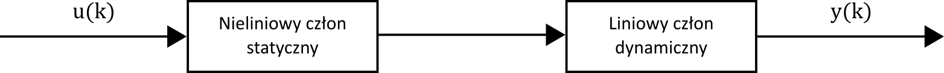
\includegraphics[width=1.0\linewidth]{hammerstein.png}
	\caption{Schemat modelu kaskadowego Hammersteina}
	\label{fig:hammerstein}
\end{figure}
W poprzednim punkcie wyznaczony został nieliniowy człon statyczny, teraz zajmiemy się liniowym członem dynamicznym. W tym celu na początek wyznaczono odpowiedź skokową z punktu pracy, zwiększając $u$ o 0,01. Wynik tego eksperymentu przedstawiono na rysunku \ref{fig:odpowiedz-skokowa}.
\begin{figure}[!h]
	\centering 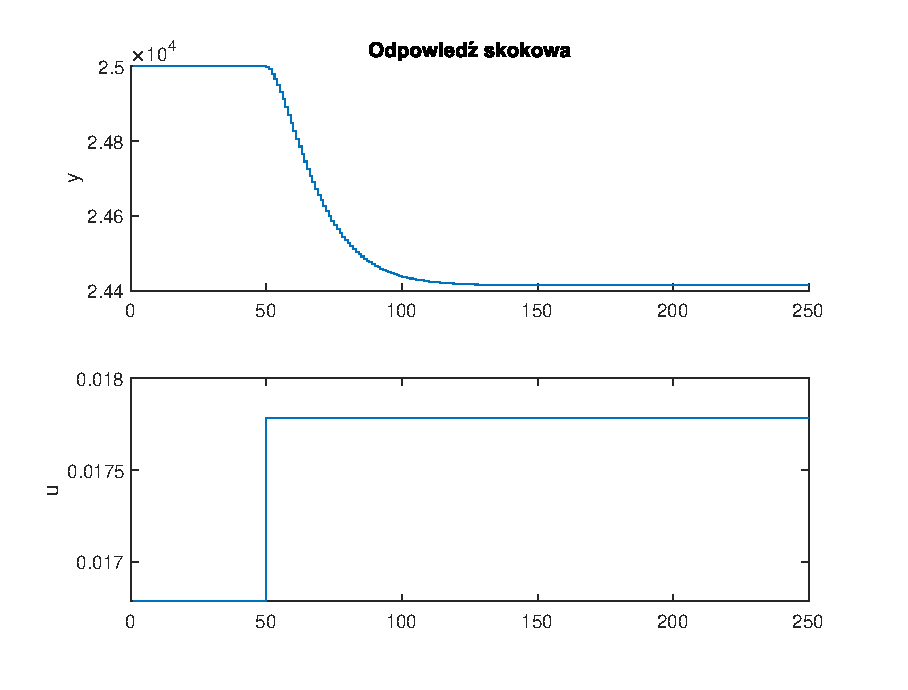
\includegraphics[width=0.8\linewidth]{odpowiedz-skokowa.eps}
	\caption{Odpowiedź skokowa obiektu}
	\label{fig:odpowiedz-skokowa}
\end{figure}
Przetestowano kilka rodzajów modelów, o różnych stopniach dynamiki, ostatecznie wybrano następujący:
\begin{equation}
\begin{split}
\hat{y}_d(k) = &a_1y(k-1) + a_2y(k-2)+a_3y(k-3)+a_4y(k-4)+ \\
+ &b_0u(k) +b_1u(k-1)+b_2u(k-2)+b_3u(k-3)+b_4u(k-4)
\end{split}
\end{equation}
Następnie poddano obróbce odpowiedź skokową, mianowicie znormalizowano skok sterowania oraz wyjście tak aby na końcu wynosiły 1. W takim przypadku wystarczy dynamikę modelu przeskalować przez nieliniowy człon statyczny otrzymując nieliniowy model dynamiczny. Po dobraniu wartości parametrów za pomocą metody najmniejszych kwadratów, przebieg wyjścia modelu przedstawiono na rysunku \ref{fig:model-dynamiczny}.
\begin{figure}[!h]
	\centering 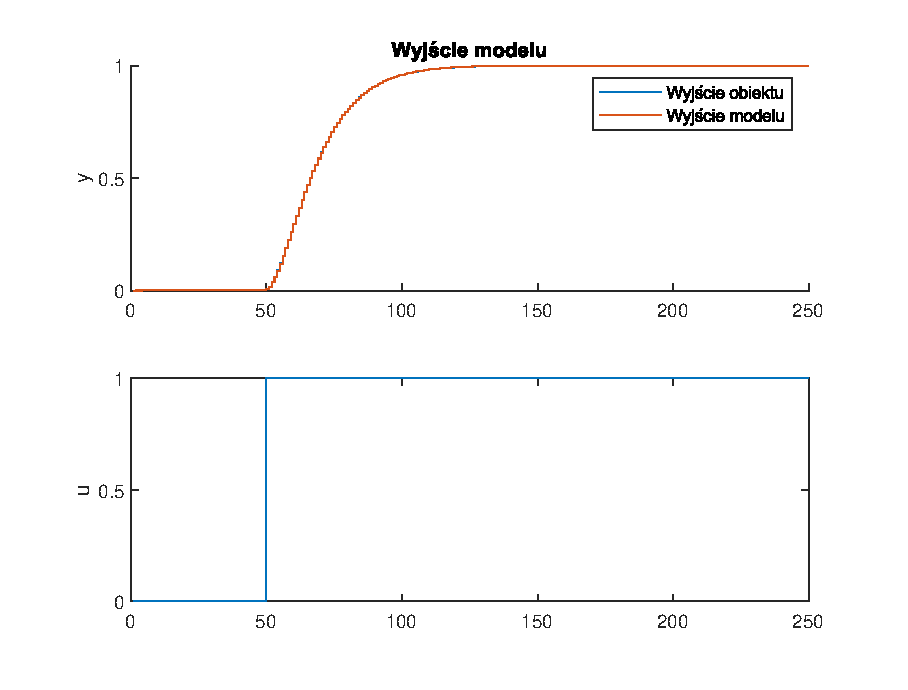
\includegraphics[width=0.8\linewidth]{model-dynamiczny.eps}
	\caption{Wyjście liniowego modelu dynamicznego}
	\label{fig:model-dynamiczny}
\end{figure}
Jak widać oba przebiegi się praktycznie pokrywają, błąd średniokwadratowy jest równy 4.1895e-08. Końcowy model będzie miał postać:
\begin{equation}
\begin{split}
\hat{y}(k) = &a_1y(k-1) + a_2y(k-2)+a_3y(k-3)+a_4y(k-4)+ \\
+ &\alpha(k) b_0u(k) +\alpha(k) b_1u(k-1)+\alpha(k) b_2u(k-2)+\alpha(k) b_3u(k-3)+\alpha(k) b_4u(k-4)
\end{split}
\end{equation}
gdzie
\begin{equation}
	\alpha(k) = \frac{\hat{y}_s(u(k))}{u(k)}
\end{equation}
Przebieg wyjściowy dla tego modelu przedstawiono na rysunku \ref{fig:przebieg-hammerstein}.
\begin{figure}[!h]
	\centering 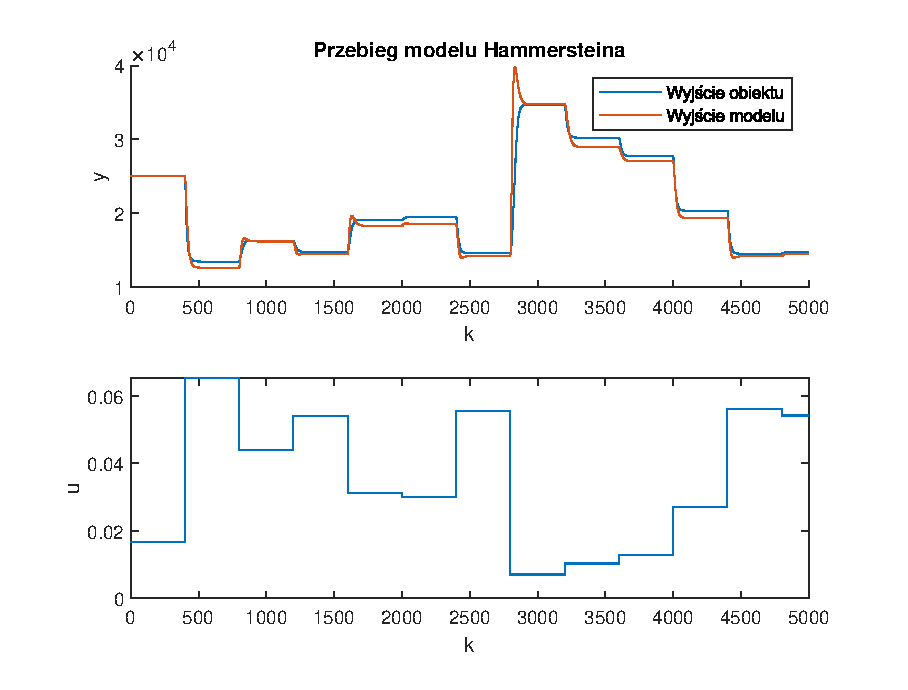
\includegraphics[width=0.8\linewidth]{przebieg-hammerstein.eps}
	\caption{Przebieg dla modelu Hammersteina}
	\label{fig:przebieg-hammerstein}
\end{figure}
Jak widać model w stanach ustalonych przyjmuje wartości statyczne wyliczone w poprzednim punkcie. Dynamika też jest w miarę dobrze odwzorowana, jednakże pojawiają się odchylenia w niektórych momentach. Może być to wina implementacji, co zostanie jeszcze zbadane w przyszłym semestrze. Błąd średniokwadratowy dla tego przebiegu był równy 6,4393e+08.